\documentclass[11pt]{article}
\usepackage{url}
\usepackage{graphicx}
\graphicspath{ {img/} }

\title{\textbf{The Topology of Sleep}}
\author{Vishnu Menon\\  
		John Jeong}
\date{}
\begin{document}

\maketitle

\section{Abstract}
In this report, we describe the results of applying Topological Data Analysis techniques to Polysomnography data (specifically, EEG waveforms). We attempt to use TDA-derived features to train classifiers for two separate Polysomnography-related tasks: identifying sleep spindles and classifying sleep stage. We describe our feature-generation and classification pipeline and consider possible sources of inaccuracy. Then, we evaluate the performance of our classifiers relative to the state-of-the-art and discuss future developments that could increase the accuracy of our approach.
  

\section{Our Dataset}
The National Institute of Neurological Disorders and Stroke estimates that over 60 million people in America alone suffer from sleep-related problems. Of these, at least 40 million suffer from chronic and long-term sleep disorders. Sleep-related medical expenses each year amount to over \$16 billion \cite{ninds}. Diagnosing and studying sleep disorders, therefore, is a major concern for many medical professionals. Polysomnography, the process of carrying out sleep studies, is often a key part of the diagnostic/exploratory process in sleep-related medical cases. A typical polysomnograph (the output of polysomnography) contains, among other signals, a patient's brainwaves, heartbeat, and breathing recorded over the course of a full night's sleep. This wealth of data often requires hours of careful analysis by trained professionals in order to interpret. Two aspects of polysomnograph data that are often measured and annotated are the positions/durations of the sleep stages/phases and the  locations of sleep spindles. 

Human sleep is divided into 5 phases: stages 1,2,3, and 4, and REM (Rapid Eye Movement) sleep. The stages vary in terms of depth of sleep, brain and muscle activity, dream activity, heart rate, and blood pressure (as well as other factors). The amount of time an individual spends in each phase can hint at various underlying issues with his or her sleep patterns; for example, patients with Sleep Apnea are often robbed of REM sleep, leaving them tired and irritable. Each sleep stage comes with distinctive EEG waveforms by which they can be identified, as shown in Figure \ref{fig:stageseeg}.

\begin{figure}[h]
    \centering
    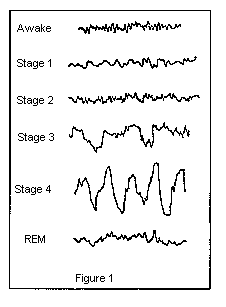
\includegraphics[width=0.25\textwidth]{sleepeeg} 
    \caption{Representative EEG waveforms from each sleep stage \cite{ninds}}
    \label{fig:stageseeg}
\end{figure}

Sleep spindles are EEG events that occur in non-REM sleep. They typically appear as "waxing-and-waning 10 $-$ 16 Hz oscillations lasting 0.5–2 s" \cite{Andrillon17821}. There are many hypotheses about their function, including suggestions that they are involved in memory, arousal, and environmental disconnection during sleep. Spindles' characteristics have also been used as an indicator for certain psychiatric disorders (including schizophrenia) \cite{Andrillon17821}.

Due to their medical relevance and their universal nature, both of these types of polysomnograph events (i.e. phases and spindles) are important to sleep specialists studying patient data. To analyze their topological characteristics, we turned to two separate datasets. The first is the DREAMS Sleep Spindle Database. This dataset consists of "8 excerpts of 30 minutes of central EEG channel (extracted from whole-night [polysomnograph] recordings), annotated independently by two experts in sleep spindles" \cite{dreams}. The excerpts vary in sampling frequency and in EEG channel used. Additionally, only 6 of the excerpts were scored by both experts, so only those 6 were used in this project. The other dataset that we utilized is the PhysioNet Sleep-EDF Database, a "collection of 61 polysomnograms (PSGs) with accompanying hypnograms (expert annotations of sleep stages) ... from two studies" \cite{kemp2000analysis}. All the EEG data in these polysomnograms is from the Fpz-Cz and Pz-Oz channels/electrode locations, and all of it is sampled at 100Hz. These two channels are used to annotate each polysomnogram with the labels W (Awake), M (Movement), ? (Uncertain), 1, 2, 3, 4, and REM; only the latter 5 labels are used in this project. 

\section{Goals} 

Given these two datasets, we hope to automate the process of identifying spindles and stages through machine learning. With sufficient accuracy, this could be helpful in a variety of medical sleep-related applications. We also hope to attain this accuracy through the use of efficiently computed TDA-based features, to validate the applicability of TDA to this space.

\section{Existing Works}

\section{Our Methods \& Results}

Our pipelines for Spindle Identification and for Stage Classification ended up being relatively similar. For spindle classification, we initially took 

\section{Future Plans}

\bibliography{bibliography} 
\bibliographystyle{acm}


\end{document}
